\section{Separability of data}
%results PCA

PCA is performed on all feature data from each test subject for both MAV and logarithmic variance features. In \figref{fig:pcasubplotMAV} a PCA is shown from one test subject, performed with the MAV feature. 

\begin{figure}[H]
	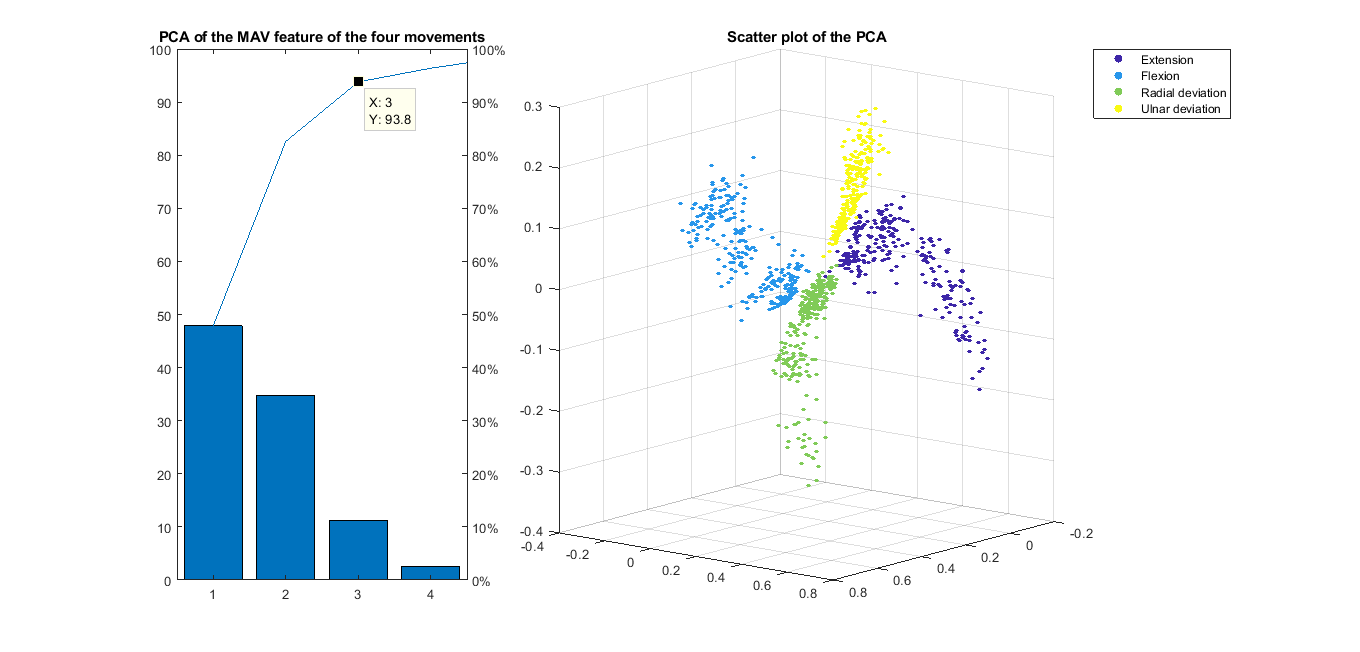
\includegraphics[height=0.2\textheight,width=1.1\textwidth]{figures/results/pcasubplotMAV.png} 
	\caption{Plot of PCA of MAV feature. To the left the first four principal components are visualised. The first three principal components account for describing $93.8\%$ of the data set. On the right the PCC's are plotted for each movement. The clusters for each movement are distinguishable from each other and have no noteworthy outliers, so the data is considered of high quality.} 
	\label{fig:pcasubplotMAV}
\end{figure} 

\begin{figure}[H]
	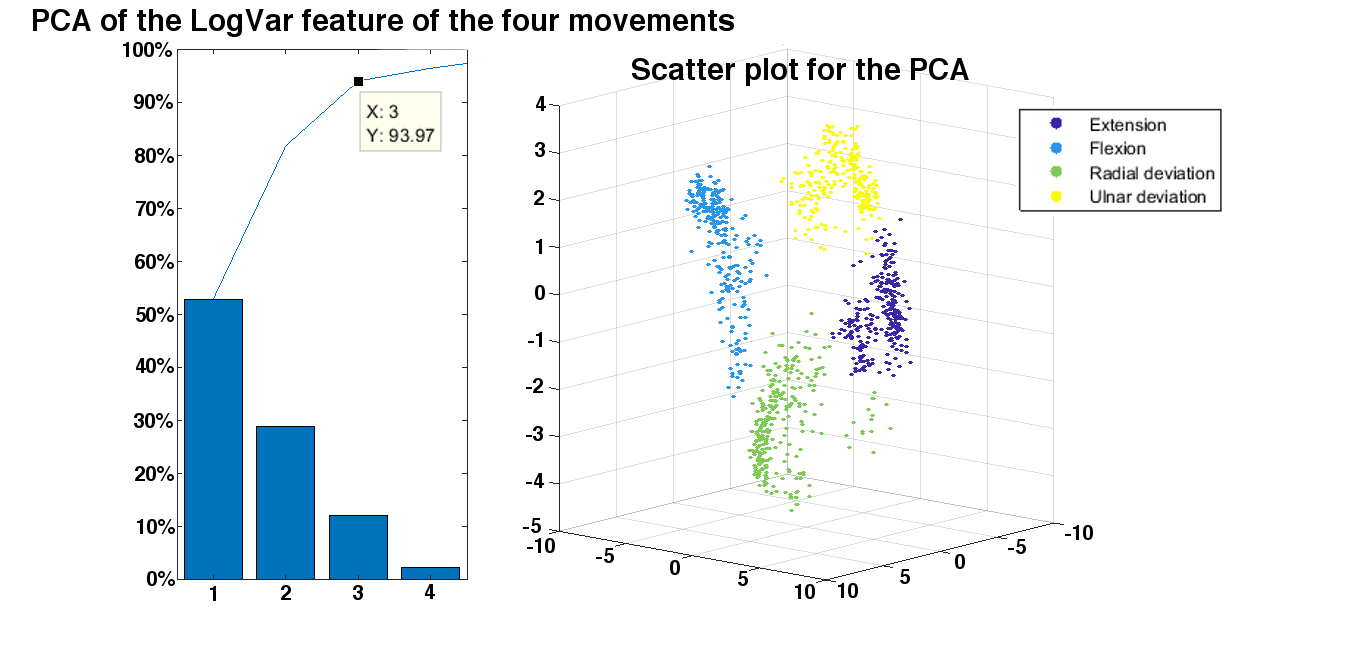
\includegraphics[height=0.2\textheight,width=1.1\textwidth]{figures/results/pcasubplotLogVar.png} 
	\caption{Plot of PCA of logarithmic variance feature. The first three principal components account for describing $93.97\%$ of the data set. Here the clusters for each movement are also distinguishable from each other and have no noteworthy outliers, so the data is considered of high quality.} 
	\label{fig:pcasubplotLogVar}
\end{figure}

The left plot of the principal components describe the importance of each identified components, and how much of the variance in the data that is described. For the MAV feature depicted in \figref{fig:pcasubplotMAV}, using only the first three components, $93.8\%$ of the full dataset can be described. Only these principal components are used in the plot to the right in both figures. The same is the case for the PCA of logarithmic variance shown in \figref{fig:pcasubplotLogVar}, where the first three PC's account for describing $93.97\%$ og the data. In both PCA's it can be seen that the clusters are easily distinguishable and have no remarkable outliers. Therefore the data is considered good and can be used in the training of the regressors.


%same with IMU data
